\chapter{Background of vision based detection}

	\section{Traditional vision algorithms}
	\label{sec:Traditional vision algorithms}
		Here we describe some tradional techniques used in computer vision. These techniques formulate some way to represent the image by encodeing various features, like corners, edges, color scheme, textures.~\cite{lee2015comparing}
		
	\subsection{\emph{SIFT(Scale invariant feature transform)}}
	
	The SIFT algorithm deals with the problem that certain image features like edges and corners are not scale-invariant. In other words, there are times when a corner looks like a corner, but looks like a completely different item when the image is blown up by a few factors. The SIFT algorithm uses a series of mathematical approximations to learn a representation of the image that is scale-invariant. In effect, it tries to standardize all images (if the image is blown up, SIFT shrinks it; if the
	image is shrunk, SIFT enlarges it). This corresponds to the
	idea that if some feature (say a corner) can be detected in an
	image using some square-window of dimension $\sigma$ across the
	pixels, then if the image was scaled to be larger, we
	would need a larger dimension k$\sigma$ to capture the same corner
	(see figure 1). The general idea is that SIFT standardizes the scale of the image then detects important key features. The existence of
	these features are subsequently encoded into a vector used to
	represent the image.
	\begin{figure}[htbp]
		\centering
		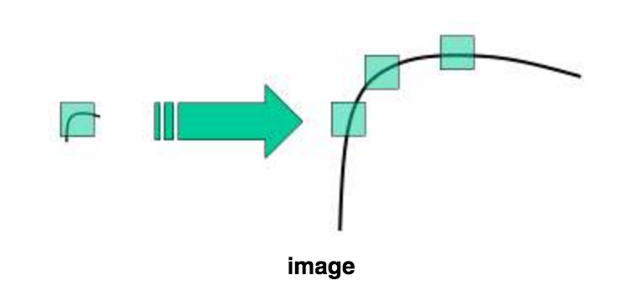
\includegraphics[width=9cm]{sift.png}
		\caption{Example showing scaling changes detection of a corner\label{Example showing scaling changes detection of a corner}}
	\end{figure}
	
	\subsection{\emph{SURF(Speeded-Up Robust Features)}}
	The problem with SIFT is that the algorithm itself uses a
	series of approximations using difference of Gaussians for standardizing the scale. Unfortunately, this approximation
	scheme is slow. SURF is simply a speeded-up version of
	SIFT. SURF works by finding a quick and dirty approximation to the difference of Gaussians using a technique called
	box blur. A box blur is the average value of all the images
	values in a given rectangle and it can be computed efficiently.
	
	\subsection{\emph{ORB(Oriented FAST and rotated BRIEF)}}
	ORB is basically a fusion of FAST keypoint detector and BRIEF descriptor with many modifications to enhance the performance. First it use FAST to find keypoints, then apply Harris corner measure to find top N points among them. It also use pyramid to produce multiscale-features. But one problem is that, FAST doesn’t compute the orientation. So what about rotation invariance? Authors came up with following modification.
	
	It computes the intensity weighted centroid of the patch with located corner at center. The direction of the vector from this corner point to centroid gives the orientation. To improve the rotation invariance, moments are computed with x and y which should be in a circular region of radius r, where r is the size of the patch.
	\begin{figure}[htbp]
		\centering
		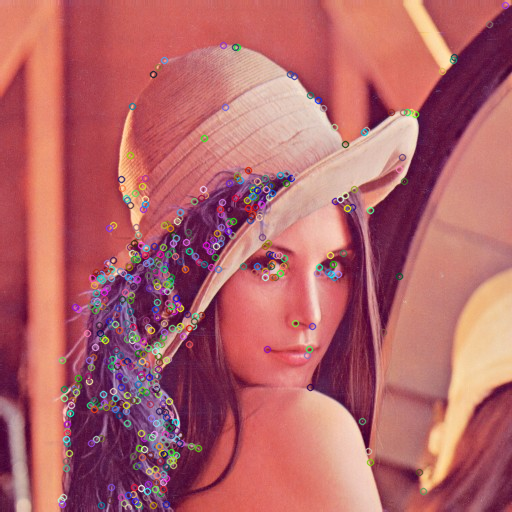
\includegraphics[width=9cm]{harris_opencv.png}
		\caption{ORB features\label{ORB features}}
	\end{figure}
	
	
	\subsection{\emph{HOG(Histogram of oriented gradients)}}
	The HOG descriptor technique counts occurrences of gradient orientation in localized portions of an image - detection window, or region of interest (ROI). Implementation of the HOG descriptor algorithm is as follows:
	
	Divide the image into small connected regions called cells, and for each cell compute a histogram of gradient directions or edge orientations for the pixels within the cell. Discretize each cell into angular bins according to the gradient orientation. Each cell's pixel contributes weighted gradient to its corresponding angular bin. Groups of adjacent cells are considered as spatial regions called blocks. The grouping of cells into a block is the basis for grouping and normalization of histograms. Normalized group of histograms represents the block histogram. The set of these block histograms represents the descriptor.
	\begin{figure}[htbp]
		\centering
		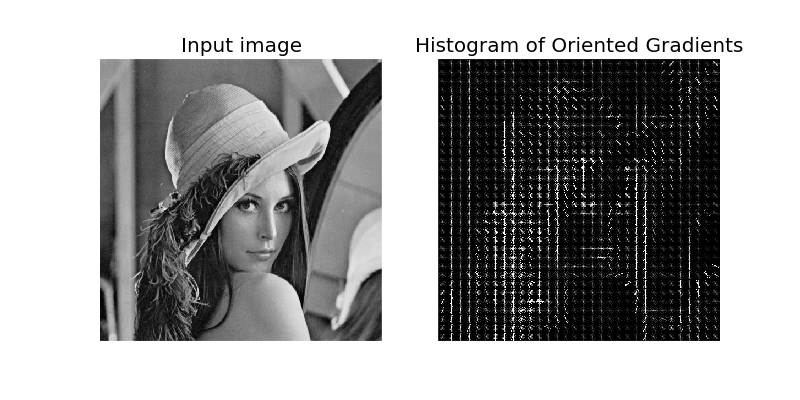
\includegraphics[width=12cm]{plot_hog.png}
		\caption{HOG features\label{HOG features}}
	\end{figure}
	
		
	\section{Deep Neural Networks}
	\label{sec:Deep Neural Networks}
		The  deep  networks  we  examine  here  are  convolutional neural networks. For those familiar with artificial neural  networks,  these are  simply  multi-level  neural  networks with a few special properties in place (pooling, convolution). The basic idea is that we will take a raw RGB image and perform a series of transformations on the image. On each transformation, we learn a denser representation of the image. We then take this denser representation, apply the transformation and learn an even further denser representation.  It turns out by using this procedure, we learn more and more abstract features with which to represent the original image.  At the end, we can use these abstract features to predict using some traditional classification method.
		\begin{figure}[htbp]
			\centering
			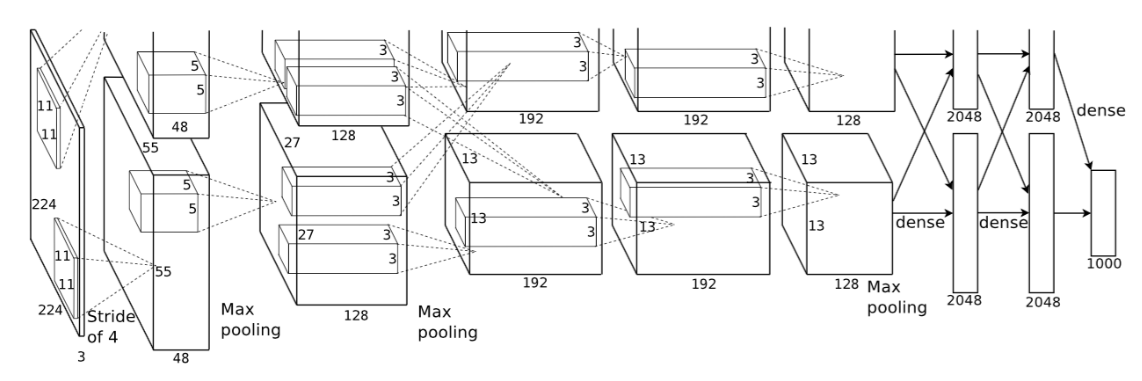
\includegraphics[width=15cm]{cnn-training.png}
			\caption{CNN training process\label{CNN training process}}
		\end{figure}
	
	\subsection{\emph{Region-based Convolutional Neural Networks(R-CNN):}}
		Since we had modeled object detection into a classification problem, success depends on the accuracy of classification. CNNs were too slow and computationally very expensive. It was impossible to run CNNs on so many patches generated by sliding window detector. R-CNN solves this problem by using an object proposal algorithm called \emph{Selective Search} which reduces the number of bounding boxes that are fed to the classifier to close to 2000 region proposals. Selective search uses local cues like texture, intensity, color or a measure of insideness etc to generate all the possible locations of the object. We feed these boxes to our CNN based classifier. Fully connected part of CNN takes a fixed sized input so, we resize(without preserving aspect ratio) all the generated boxes to a fixed size (224 x 224 for VGG) and feed to the CNN part. Hence, there are 3 important parts of R-CNN:~\cite{objdet}
		
		\begin{itemize}
			\item Run Selective Search to generate probable objects.
			\item Feed these patches to CNN, followed by SVM to predict the class of each patch.
			\item Optimize patches by training bounding box regression separately.
		\end{itemize}
		
		\begin{figure}[htbp]
			\centering
			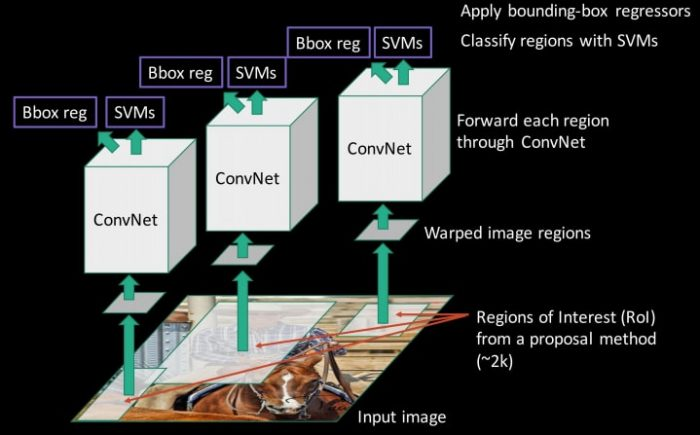
\includegraphics[width=12cm]{rcnn2.jpg}
			\caption{R-CNN\label{R-CNN}}
		\end{figure}
		
		
	\subsection{\emph{Spatial Pyramid Pooling(SPP-net):}}
		Still, RCNN was very slow. Because running CNN on 2000 region proposals generated by Selective search takes a lot of time. SPP-Net tried to fix this. With SPP-net, we calculate the CNN representation for entire image only once and can use that to calculate the CNN representation for each patch generated by Selective Search. This can be done by performing a pooling type of operation on JUST that section of the feature maps of last conv layer that corresponds to the region. The rectangular section of conv layer corresponding to a region can be calculated by projecting the region on conv layer by taking into account the downsampling happening in the intermediate layers(simply dividing the coordinates by 16 in case of VGG). 
		
		We need to generate the fixed size of input for the fully connected layers of the CNN so, SPP introduces one more trick. It uses spatial pooling after the last convolutional layer as opposed to traditionally used max-pooling. SPP layer divides a region of any arbitrary size into a constant number of bins and max pool is performed on each of the bins. Since the number of bins remains the same, a constant size vector is produced as demonstrated in the figure below.
		\begin{figure}[htbp]
			\centering
			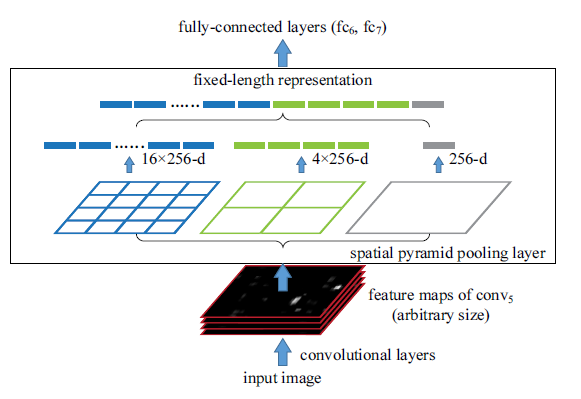
\includegraphics[width=12cm]{spp-nn.png}
			\caption{SPP-net\label{SPP-net}}
		\end{figure}
		There was one big drawback with SPP net, it was not trivial to perform back-propagation through spatial pooling layer. Hence, the network only fine-tuned the fully connected part of the network. SPP-Net paved the way for more popular Fast RCNN.
		
	\subsection{\emph{Fast R-CNN}}
		Fast RCNN uses the ideas from SPP-net and RCNN and fixes the key problem in SPP-net i.e. they made it possible to train end-to-end. To propagate the gradients through spatial pooling,  It uses a simple back-propagation calculation which is very similar to max-pooling gradient calculation with the exception that pooling regions overlap and therefore a cell can have gradients pumping in from multiple regions.
		
		One more thing that Fast RCNN did that they added the bounding box regression to the neural network training itself. So, now the network had two heads, classification head, and bounding box regression head. This multitask objective is a salient feature of Fast-rcnn as it no longer requires training of the network independently for classification and localization. These two changes reduce the overall training time and increase the accuracy in comparison to SPP net because of the end to end learning of CNN.
		
	\subsection{\emph{Faster R-CNN}}
		Faster RCNN replaces selective search with a very small convolutional network called Region Proposal Network to generate regions of Interests.~\cite{ren2015faster}
		\begin{figure}[htbp]
			\centering
			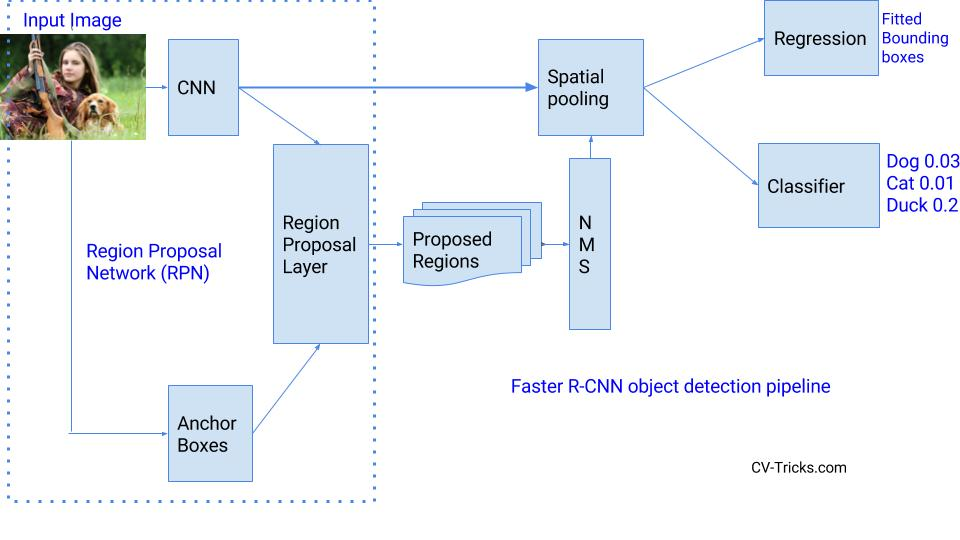
\includegraphics[width=15cm]{Faster-RCNN.jpg}
			\caption{Faster R-CNN object detecttion pipeline\label{Faster R-CNN object detecttion pipeline}}
		\end{figure}
		
		To handle the variations in aspect ratio and scale of objects, Faster R-CNN introduces the idea of \emph{anchor boxes}. At each location, the original paper uses 3 kinds of anchor boxes for scale \emph{128*128, 256*256 and 512*512}. Similarly, for aspect ratio, it uses three aspect ratios \emph{1:1, 2:1 and 1:2}. So, in total at each location, we have 9 boxes on which RPN predicts the probability of it being background or foreground. We apply bounding box regression to improve the anchor boxes at each location. So, RPN gives out bounding boxes of various sizes with the corresponding probabilities of each class. The varying sizes of bounding boxes can be passed further by applying Spatial Pooling just like Fast-RCNN. The remaining network is similar to Fast-RCNN. Faster-RCNN is 10 times faster than Fast-RCNN with similar accuracy of datasets like VOC-2007. That’s why Faster-RCNN has been one of the most accurate object detection algorithms. Here is a quick comparison between various versions of RCNN.
		\begin{table}[h!]
			\centering
			\begin{tabular}{| c | c | c | c |}
				\hline
				Category	& R-CNN & Fast R-CNN	& Faster R-CNN	\\ \hline  \hline
				Test time per image		& 50s	& 2s	& 0.2s\\ \hline
				Speed Up	& 1x	& 25x	& 250x\\ \hline
			\end{tabular}
			\caption{Comparison between various R-CNNs}
			\label{table:Comparison between various R-CNNsTime Analysis}
		\end{table}
	
	
	\subsection{\emph{YOLO(You only Look Once):}}
		 YOLO divides each image into a grid of S x S and each grid predicts N bounding boxes and confidence. The confidence reflects the accuracy of the bounding box and whether the bounding box actually contains an object(regardless of class). YOLO also predicts the classification score for each box for every class in training. We can combine both the classes to calculate the probability of each class being present in a predicted box.~\cite{objdet}
		 
		 So, total SxSxN boxes are predicted. However, most of these boxes have low confidence scores and if we set a threshold say 30 percent confidence, we can remove most of them as shown in the example below.
		 \begin{figure}[htbp]
		 	\centering
		 	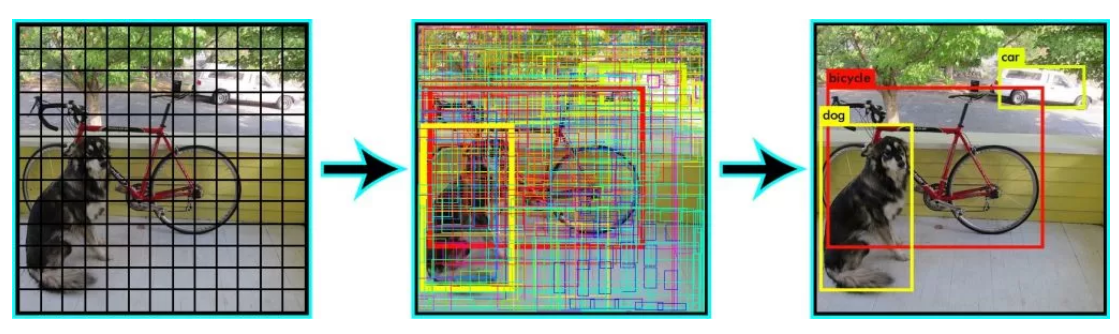
\includegraphics[width=15cm]{yolo.PNG}
		 	\caption{YOLO model\label{YOLO model}}
		 \end{figure}
		 
		 At runtime, we have run our image on CNN only once. Hence, YOLO is super fast and can be run real time. Another key difference is that YOLO sees the complete image at once as opposed to looking at only a generated region proposals in the previous methods. So, this contextual information helps in avoiding false positives. However, one limitation for YOLO is that it only predicts 1 type of class in one grid hence, it struggles with very small objects. 
		  
	\subsection{\emph{Single Shot Detector(SSD):}}
		Single Shot Detector achieves a good balance between speed and accuracy. SSD runs a convolutional network on input image only once and calculates a feature map. Now, we run a small 3×3 sized convolutional kernel on this feature map to predict the bounding boxes and classification probability. SSD also uses anchor boxes at various aspect ratio similar to Faster-RCNN and learns the off-set rather than learning the box. In order to handle the scale, SSD predicts bounding boxes after multiple convolutional layers. Since each convolutional layer operates at a different scale, it is able to detect objects of various scales. ~\cite{objdet}
	
	\section{Relevant literature}
	\label{sec:Relevant Literature}
	
	\subsection{ImageNet Classification with Deep Convolutional Neural Networks}
		This paper discusses a neural network containing over 60 million parameters and 60 million parameters that significantly beat previous state-of-the-art approaches to image recognition in a popular computer
		vision competition: ISVRC-2012
		
		The architecture of the featured convolutional neural network is given by 5 convolutional layers that are followed by  max-pooling  layers  and  3  full-connected layers with a final 1000-way softmax. Important innovations of this paper include  an  alternative to  the  traditional  sigmoid  activation function and methods for reducing over-fitting. Traditionally,
		activation functions take the form
		
		\begin{equation}
		f(x) = (1+e^{-x})^{-1} \quad or\quad tanh(x)
		\end{equation}
		
		However, the paper advocates the use of \emph{Rectified Linear Units (ReLUs)}, which refers to the activation function
		
		\begin{equation}f(x) = max(0,x) \end{equation}
		
		The max function significantly accelerates learning time. To
		reduce over-fitting, the authors also artificially enlarged the
		data set by generating image translations and horizontal reflections on each image, while preserving their labels. This
		increased the training set by a factor of 2048. While the new
		training examples are highly correlated with the original examples, this data augmentation forces the network to learn multiple representations of the same image, thereby encouraging generalization. CNN described in this paper achieves an error rate of 37.5 as compared to a more traditional approach of using SIFT + FV features, which achieves an error rate of 45.7.
		~\cite{lee2015comparing}
	
	\section{Comparison Results}
	\label{sec:Comparison Results}
		
		 Currently, Faster-RCNN is the choice if we are concerned about accuracy numbers. However, if we require  better computation(probably running it on Nvidia Jetsons), SSD is a better recommendation. Finally, if accuracy is not too much of a concern but we want to go super fast, YOLO will be the way to go. First of all a visual understanding of speed vs accuracy trade-off can be found in Figure 3.9.~\cite{objdet}
		
		\begin{figure}[htb]
			\centering
			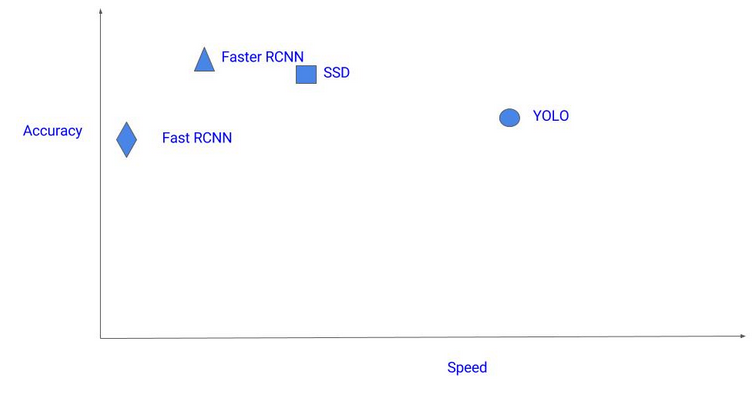
\includegraphics[width=14cm]{speed.png}
			\caption{YOLO vs SSD\label{YOLO vs SSD}}
		\end{figure}
		
		SSD seems to be a good choice as we are able to run it on a video and the accuracy trade-off is very little. This chart compares the performance of SSD, YOLO, and Faster-RCNN on various sized objects. At large sizes, SSD seems to perform similarly to Faster-RCNN. However, when we look at the accuracy numbers for smaller sized objects, the gap widens, as seen in Fig 3.10.
		
		\begin{figure}[ht!]
			\centering
			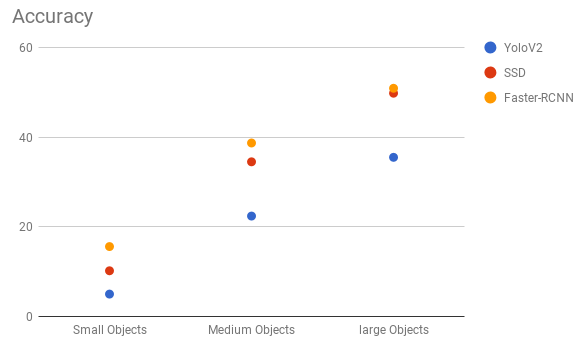
\includegraphics[width=14cm]{accuracy.png}
			\caption{YOLO vs SSD(Based on Object size)\label{YOLO vs SSD}}
		\end{figure}
		
		This choice of a right object detection method is crucial and depends on the problem that we are trying to solve and the set-up. Object Detection is the backbone of many practical applications of computer vision such as autonomous cars, security and surveillance, and many other industrial and domestic applications.
		
		In order to solve the problem in this thesis, we have used a SSD based Tensorflow object detection API released some time back.
		
		
		
		
		